\documentclass[10pt]{article}
\usepackage{tikz}
\usetikzlibrary{shapes.misc}
\usepackage[margin=0cm]{geometry}
\pagestyle{empty}
\tikzstyle{every node}=[cross out, draw, red]

\begin{document}

\vspace*{\fill}
\begin{center}
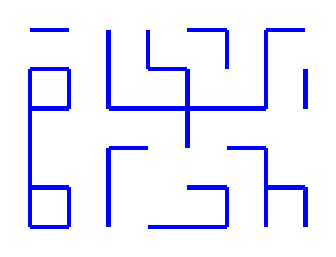
\begin{tikzpicture}[x=0.5cm, y=-0.5cm, ultra thick, blue]
% Walls
    \draw (0,0) -- (1,0);
    \draw (2,0) -- (2,1);
    \draw (3,0) -- (3,1);
    \draw (4,0) -- (5,0);
    \draw (5,0) -- (5,1);
    \draw (6,0) -- (6,1);
    \draw (6,0) -- (7,0);
    \draw (0,1) -- (0,2);
    \draw (0,1) -- (1,1);
    \draw (1,1) -- (1,2);
    \draw (2,1) -- (2,2);
    \draw (3,1) -- (4,1);
    \draw (4,1) -- (4,2);
    \draw (6,1) -- (6,2);
    \draw (7,1) -- (7,2);
    \draw (0,2) -- (0,3);
    \draw (0,2) -- (1,2);
    \draw (2,2) -- (3,2);
    \draw (3,2) -- (4,2);
    \draw (4,2) -- (4,3);
    \draw (4,2) -- (5,2);
    \draw (5,2) -- (6,2);
    \draw (0,3) -- (0,4);
    \draw (2,3) -- (2,4);
    \draw (2,3) -- (3,3);
    \draw (5,3) -- (6,3);
    \draw (6,3) -- (6,4);
    \draw (0,4) -- (0,5);
    \draw (0,4) -- (1,4);
    \draw (1,4) -- (1,5);
    \draw (2,4) -- (2,5);
    \draw (4,4) -- (5,4);
    \draw (5,4) -- (5,5);
    \draw (6,4) -- (6,5);
    \draw (6,4) -- (7,4);
    \draw (7,4) -- (7,5);
    \draw (0,5) -- (1,5);
    \draw (3,5) -- (4,5);
    \draw (4,5) -- (5,5);

\end{tikzpicture}
\end{center}
\vspace*{\fill}

\end{document}
